\documentclass[12pt]{article}
\usepackage{graphicx} % Required for inserting images
\usepackage{geometry}
\usepackage[T1]{fontenc}
\usepackage[utf8]{inputenc}
\usepackage{float}
\usepackage{hyperref}
\usepackage{listings}
\usepackage{xcolor}
\usepackage{fancybox}
\usepackage[most]{tcolorbox} 

\renewcommand{\figurename}{Slika}
\renewcommand{\baselinestretch}{1.2} % Line spacing

% Define a command to ensure the new section starts on an odd page
\newcommand{\startnewsection}{
    \clearpage % Ends the current page
    \ifodd\value{page}\else % Check if the current page is odd
        \hbox{} % Create an empty box
        \newpage % Force a new page if the current page is even
    \fi
}

\usepackage[
   backend=biber,
   style=numeric,
   sorting=none
   ]{biblatex}

\addbibresource{references.bib}
\AtBeginBibliography{\vspace*{10pt}}


% Define custom colors
\definecolor{darkgreen}{rgb}{0.0, 0.5, 0.0} % Custom dark green color
\definecolor{grayborder}{rgb}{0.6, 0.6, 0.6} % Custom gray color for the border

\lstdefinelanguage{JavaScript}{
  keywords={break, case, catch, continue, debugger, default, delete, do, else, finally, for, function, if, in, instanceof, new, return, switch, this, throw, try, typeof, var, void, while, with, let, const, await, async},
  sensitive=true,
  comment=[l]{//},
  morecomment=[s]{/*}{*/},
  morestring=[b]',
  morestring=[b]",
  keywordstyle=\color{blue}\bfseries,
  commentstyle=\color{gray}\itshape,
  stringstyle=\color{darkgreen}, % Changed to a darker green
}

\lstset{
  language=JavaScript,
  basicstyle=\scriptsize\ttfamily, % Make font size smaller
  keywordstyle=\color{blue}\bfseries,
  commentstyle=\color{gray}\itshape,
  stringstyle=\color{darkgreen},
  numberstyle=\tiny\color{gray},
  stepnumber=1,
  showstringspaces=false,
  tabsize=2
}

% Define a tcolorbox style for listings
\newtcolorbox[auto counter, number within=section]{mylisting}[2][]{colback=white!10!white, colframe=grayborder,
  fonttitle=\bfseries, title=Listing~\thetcbcounter: #2,#1}


\title{Bachelor Thesis}
\author{Ivan Jevtic}
\date{September 2024}

\begin{document}

% Title Page
\newgeometry{top=1in, bottom=1in, left=1in, right=1in} % New margins for title page
\begin{titlepage}
	\begin{center}
		         
		% add your university logo here
		% negative value moves the logo up
		\vspace*{-1in}
		\includegraphics[width=0.4\textwidth]{raf_logo.png}
		
		% set font size to 14pt
		\vspace{1in}
		\Large
		\textbf{DIPLOMSKI RAD}
		         
		% set horizontal margin for the title to 1.5in and center it
		\vspace{1in}
		\Huge
		\textbf{Razvoj višekorisničkog kolaborativnog editora}
		         
		\vspace{1in}
		
		
		\fontsize{14pt}{18pt}\selectfont
		\textbf{Ivan Jevtić} \\
		\textbf{RN 4/2020}
		\vspace*{1.5in}
		         
		\begin{center}
			\normalsize
			\begin{tabular}{p{0.7\textwidth} p{0.5\textwidth}}
				\fontsize{14pt}{18pt}\selectfont   
				\textbf{Mentor:}      &                       
				            
				\fontsize{14pt}{18pt}\selectfont
				\textbf{Komisija:} \\
				dr Miloš Radenković &  \\
				                                 
			\end{tabular}
		\end{center}
		
		\vspace*{\fill}
		
		\normalsize
		Beograd, septembar 2024.
		
		
		         
	\end{center}
\end{titlepage}
\restoregeometry % Restore original margins

\newpage
\newgeometry{top=1.3in, bottom=2.2in, left=1.4in, right=1.4in} % New margins for title page
   
% Table of Contents
\renewcommand{\contentsname}{Sadržaj}
\addtocontents{toc}{\protect\thispagestyle{empty}}
\tableofcontents
\thispagestyle{empty} % Remove page numbers

\restoregeometry % Restore original margins

\newpage
   
\thispagestyle{empty} % Remove page number from Abstract page
    
% Define a command to format a specific section title
\newcommand{\specialsection}[1]{
	\section*{\centering{#1}} % Center and italicize the section title
}
    
\vspace*{0.5in}
\specialsection{Apstrakt}
    
\vspace*{0.5in}

Here is a reference to the work by Sousa \cite{sousa2012} and by Finn \cite{finn2016}.

Ovaj diplomski rad istražuje \textbf{višekorisničke kolaborativne editore}, sisteme koji omogućavaju istovremenu saradnju više korisnika na istom dokumentu u realnom vremenu. U uvodnom delu rada, pružen je detaljan pregled osnovnih principa ovih sistema i kratak istorijat razvijanja kolaborativnih editora.

Detaljno su opisana dva algoritma za automatsko rešavanje konflikata kod kolaborativnih editora, a to su \textbf{Operational Transformation} i \textbf{Conflict-free Replicated Data Types}.

Rad se zatim fokusira na razvoj prilagođenog višekorisničkog kolaborativnog editora. Opisuje se \textbf{arhitektura rešenja} i korišćeni \textbf{algoritmi} za sinhronizaciju podataka. Takođe, analizirani su postojeći alati i rešenja, kao što su \textbf{Etherpad}\cite{etherpad} i \textbf{Firepad}\cite{firepad}, zajedno sa njihovim prednostima i manama.

\newpage

\newpage
\pagenumbering{arabic}
\setcounter{page}{1}

\startnewsection

\section{Uvod}

\vspace{+0.5cm}
   
\subsection{Definicija}

\subsubsection{Kolaborativno uređivanje}

Kolaborativno uređivanje je proces u kojem više ljudi istovremeno radi na istom dokumentu. Ovakav pristup omogućava da različiti stručnjaci doprinesu sadržaju, što može poboljšati kvalitet dokumenta i ubrzati proces rada.

Važno je strateški odabrati najbolji pristup kako bi se postigla potpuna svest o tome ko doprinosi dokumentu, neometana koordinacija rada i aktivno učešće svih članova tima. Na primer, pisanje može biti precizno podeljeno na zadatke, gde svaki član grupe ima svoj specifičan deo, ili svi mogu sinhronizovano raditi zajedno na istom zadatku. Ovaj dinamičan proces obuhvata detaljno planiranje, inspirativno pisanje i temeljnu reviziju, pri čemu je više ljudi strateški uključeno u barem jednu od faza. Odluke o strukturi i sadržaju dokumenta uglavnom se donose zajednički kroz konstruktivnu i uključivu diskusiju unutar tima.
    
Najčešće se kolaborativno uređivanje primenjuje na tekstualne dokumente ili programski kod. Asinhroni doprinosi članova su korisni jer ne moraju svi raditi u isto vreme, što štedi vreme. Takav rad obično zahteva specijalan softver. Tekstualni procesori takođe omogućavaju beleženje izmena, što omogućava pregled ko je i šta promenio u dokumentu. Moderni alati kao što su Google Docs nude funkcije za kolaborativno pisanje i uređivanje u realnom vremenu, sa mogućnošću sinhronog i asinhronog rada.

Kolaborativno uređivanje postoji u dva formata - sinhrono i asinhrono.

Kod \textbf{asinhronog} uređivanja promene se ne sinhronizuju u realnom vremenu. Korisnici mogu istovremeno da uređuju svoje kopije, ali da bi se sinhronizovale sa serverom i drugim klijentima, moraće da ručno izvrše ažuriranje promena. Sistem sam upravlja rešavanjem konflikata, spaja više izmena i dovodi kopiju u dosledno stanje.Nekada je potrebno da korisnik pomogne u rešavanju konflikata. Sve tehnologije za kontrolu verzija kao što su Git, CVS, Subversion itd. spadaju u ovu tehnologiju.

Kod \textbf{sinhronog} uređivanja promene se sinhronizuju u realnom vremenu. Korisnici mogu istovremeno da uređuju svoje kopije, ali će takođe odmah videti promene koje su napravili drugi klijenti. Korisnici nisu obavezni da ručno izvrše komitovanje ili ažuriranje promena, sistem to radi automatski. Sistem preuzima potpunu odgovornost za rešavanje konflikata, spajajući više izmena i dovodeći dokument u dosledno stanje. Ovaj koncept je popularizovan proizvodom pod nazivom Writely, koji je nudio uređivanje u pregledaču. Kupio ga je Google 2006. godine i pretvorio u Google Docs.
    
\subsubsection{Višekorisnički kolaborativni editor}

Višekorisnički kolaborativni editor je alat koji omogućava više korisnika da istovremeno uređuju jedan isti dokument u realnom vremenu. Ovi editori su specifično dizajnirani da omoguće nesmetanu i efikasnu kolaboraciju, bez obzira na fizičku lokaciju učesnika. Ključne karakteristike ovakvih sistema uključuju sinhronizaciju izmena, kontrolu verzija i uvid u promene koje svaki korisnik napravi, uz minimalna kašnjenja ili konflikte.

\paragraph {Glavne karakteristike višekorisničkih kolaborativnih editora}
    
\begin{itemize}
	\item \textbf{Real-time sinhronizacija}: Sve izmene koje jedan korisnik napravi trenutno su vidljive ostalim korisnicima, bez potrebe za manuelnim osvežavanjem ili slanjem dokumenata.
	\item \textbf{Istovremena izmena}: Više korisnika može uređivati isti dokument ili čak isti deo dokumenta u isto vreme.
	\item \textbf{Praćenje promena}: Alat omogućava da se vidi ko je napravio koju promenu, olakšavajući timovima da prate napredak i diskutuju o izmenama.
	\item \textbf{Kontrola verzija}: Većina ovih alata poseduje sistem za praćenje verzija, koji omogućava vraćanje na prethodne verzije dokumenta, ukoliko je to potrebno.
	\item \textbf{Obaveštenja i komentarisanje}: Uključena su i obaveštenja o izmenama i mogućnost ostavljanja komentara na određene delove dokumenta, što pomaže u komunikaciji između učesnika.
	\item \textbf{Upravljanje pristupom}: Urednici mogu imati različite nivoe pristupa (npr. samo za čitanje ili za uređivanje), čime se osigurava da samo određeni korisnici mogu menjati sadržaj.
\end{itemize}

Ovi editori su nezamenjivi u okruženjima gde je potrebno brzo donošenje odluka i rad na zajedničkim dokumentima, kao što su timski projekti, akademski radovi ili kodiranje softvera.

\subsection{Istorija i motivacija}
   

\subsubsection{Rani razvoj kolaborativnih editora (1970-1980)}

Ideja kolaborativnih editora, koji omogućavaju više korisnika da istovremeno rade na istom dokumentu, počela je da se razvija tokom 1970-ih godina, u vreme kada su naučnici i inženjeri počeli da istražuju potencijal multi-korisničkih sistema. Ova era bila je obeležena pionirskim radom na sistemima koji su nastojali da olakšaju istovremenu saradnju između korisnika, mada je razvoj tih tehnologija bio ograničen dostupnim resursima, kao što su niska brzina mrežnih veza i ograničena računska snaga.
    
Jedan od prvih važnih koraka u ovom pravcu bio je razvoj \textbf{NLS sistema (oN-Line System)}, koji je predstavio \textbf{Daglas Engelbart} 1968. godine.

\paragraph{}
\textbf{NLS sistem}, poznat kao \textbf{oN-Line System (NLS)}, razvijen je zahvaljujući finansiranju od strane DARPA-e i Ratnog vazduhoplovstva SAD-a. NLS je zamišljen od strane \textbf{Daglasa Engelbarta} i razvijen u saradnji sa njegovim kolegama iz \textbf{Stanford Research Institute} (SRI). Ovaj sistem je prvi uveo koncept \textbf{hipertekstualnih linkova}, \textbf{miša}, \textbf{raster-sken monitora}, organizaciju informacija po relevantnosti, \textbf{prozor na ekranu} (windowing), prezentacione programe i mnoge druge koncepte koji su danas sastavni deo savremenih računarskih sistema. \cite{gerritsen1992}
    
Dana \textbf{9. decembra 1968.}, Engelbart je javnosti predstavio NLS sistem u San Francisku, na \textbf{Fall Joint Computer Conference}, događaju koji je kasnije postao poznat kao \textit{"Majka svih demonstracija"} zbog brojnih revolucionarnih funkcija koje su tom prilikom prvi put prikazane. Engelbartov terminal bio je povezan sa video projekcijom velikog formata, pozajmljenom od NASA Ames Research Center, a putem telefonskih linija povezan je sa SDS 940 računarom u Menlo Parku, Kalifornija, na udaljenosti od 30 milja, gde se nalazio \textbf{Augmentation Research Center}, koji je Engelbart osnovao u SRI.
    
Na ekranu visokom skoro \textbf{7 metara}, sa video umecima, publika je mogla da vidi kako Engelbart upravlja mišem, dok su se članovi njegovog tima iz Menlo Parka pridruživali prezentaciji u realnom vremenu. Dolaskom ARPA mreže u SRI 1969. godine, tehnologija vremenskog deljenja resursa (time-sharing) postala je nepraktična za distribuciju među većim brojem korisnika, ali je NLS otvorio put ka razvoju savremenih informacionih tehnologija koje danas koristimo.
    
\begin{figure}[h]
	\centering
	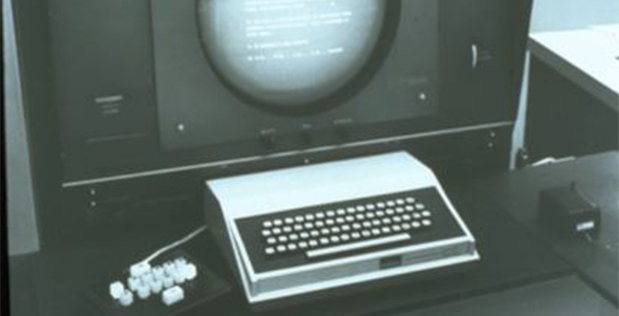
\includegraphics[width=0.8\textwidth]{nls.jpg}
	\caption{Daglas Engelbart tokom "Majke svih demonstracija", 1968.}
	
\end{figure}

    
Iako NLS nije bio kolaborativni editor u savremenom smislu, predstavljao je revolucionaran koncept koji je omogućavao zajedničko pregledanje i uređivanje dokumenata. Ovaj sistem je pokazao kako bi računar mogao postati alat za grupni rad, posebno u organizacijama sa složenim informacionim potrebama. Engelbartova vizija o umreženoj saradnji postavila je temelj za dalji razvoj kolaborativnih editora, ali su tehnološka ograničenja tog vremena sprečila njegovu široku primenu.
    
U toku 1970-ih i ranih 1980-ih, nekoliko naučnih radova i istraživanja pokušalo je da reši problem zajedničkog uređivanja dokumenata. Međutim, zbog ograničenih mrežnih kapaciteta i činjenice da internet još uvek nije bio široko dostupan, razvoj je bio fokusiran na lokalne mreže i eksperimentalne sisteme. Primer toga bio je konceptualni okvir poznat kao \textbf{"Shared Workspace"}, koji je omogućavao korisnicima da dele radno okruženje i informacije u realnom vremenu. Ovi rani sistemi su omogućavali deljenje sadržaja, ali nisu nudili dinamičko uređivanje, koje je karakteristično za modernu kolaboraciju.

\paragraph{}
Tokom kasnih 1980-ih, tehnologija je značajno napredovala, a računarstvo je postajalo sve moćnije i pristupačnije. Ova era je videla pojavu prvih pravih kolaborativnih editora. Jedan od prvih sistema koji je omogućio više korisnika da uređuju dokumente u realnom vremenu bio je \textbf{GROVE (Group Outline Viewing Editor)}, razvijen 1989. godine. GROVE je omogućavao simultano uređivanje strukturisanih dokumenata i predstavljao je jedan od pionirskih sistema za kolaborativno uređivanje. Iako je bio ograničen na lokalne mreže, zbog nedostatka interneta i infrastrukture za širu mrežnu primenu, GROVE je pokazao kako bi kolaboracija mogla funkcionisati u okruženju sa više korisnika.\cite{sibbet2024}

GROVE omogućava prikazivanje više pogleda na konturu, gde se svaki prikaz prikazuje u grupnom prozoru koji može biti repliciran na više mašina. Ovi prikazi mogu biti privatni, deljeni ili javni, u zavisnosti od potreba korisnika. Značajna karakteristika GROVE sistema je njegov grupni prozor, koji prikazuje prisustvo i aktivnost svih učesnika koji rade na dokumentu. U ovom zajedničkom prostoru korisnici mogu izvršavati standardne operacije uređivanja, kao što su umetanje, brisanje, sečenje i lepljenje teksta. Sistem takođe nudi napredne funkcionalnosti, poput proširivanja i skupljanja delova konture, kao i promene dozvola za čitanje i pisanje specifičnih stavki.

\begin{figure}[h]
	\centering
	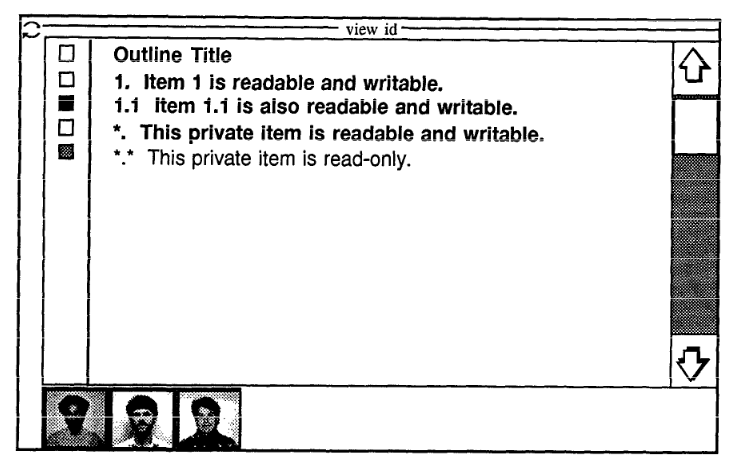
\includegraphics[width=0.8\textwidth]{grove.png}
	\caption{Grove grupni prozor, 1989.}
	
\end{figure}

Jedna od ključnih karakteristika GROVE sistema je kolaboracija u realnom vremenu—svaka promena koju napravi jedan učesnik odmah je vidljiva ostalima, osiguravajući da svi učesnici budu u toku sa najnovijim izmenama. Ovaj mehanizam povratne informacije u realnom vremenu bio je od suštinskog značaja za kreiranje visoko interaktivnog i responzivnog okruženja.
    
Za razliku od sistema u realnom vremenu kao što je GROVE, drugi sistemi tog vremena, poput CES-a, Quilta ili Shared Books-a, omogućavali su kolaborativno uređivanje dokumenata, ali su radili u asinhronom režimu. Ovi sistemi su dozvoljavali korisnicima da rade na različitim delovima dokumenta, često tokom dužih perioda, što je omogućavalo manje fokusirane sesije. Distinkcija između kolaborativnih sistema u realnom i asinhronom vremenu postala je važan fokus u proučavanju kolaborativnih sistema.
    
GROVE-ova mogućnost uređivanja u realnom vremenu, uz podršku za upravljanje različitim prikazima i korisničkim dozvolama, učinila ga je značajnim korakom u razvoju sistema za grupni rad.
    
Pored GROVE-a, nekoliko drugih projekata je nastalo u ovom periodu, ali su svi imali slične izazove – mrežna infrastruktura nije bila dovoljno razvijena za globalnu kolaboraciju, a računarstvo nije bilo dovoljno moćno da podrži složene algoritme potrebne za rešavanje problema sinkronizacije i konzistentnosti podataka među korisnicima.
    
Dakle, tokom 1970-ih i 1980-ih godina, iako su načinjeni značajni koraci u pravcu kolaborativnih sistema, ovi rani pokušaji su uglavnom ostali ograničeni na istraživačke laboratorije i specifične upotrebe unutar lokalnih mreža. Tek kasnije, sa razvojem interneta i većom dostupnošću mrežnih resursa, kolaborativni editori su počeli da ostvaruju svoj puni potencijal.

\subsubsection{Razvoj real-time kolaboracije (2000-te)}

Početak 2000-ih godina doneo je velike promene u načinu na koji ljudi rade zajedno, zahvaljujući razvoju interneta i novih tehnologija za kolaborativno uređivanje. Prethodne decenije, kolaborativni editori su postojali, ali su bili uglavnom ograničeni na lokalne mreže i zahtevali su specifične softverske sisteme. Sa ekspanzijom interneta, pojavile su se mogućnosti za udaljenu, real-time saradnju, što je omogućilo korisnicima da rade na istom dokumentu bez obzira na to gde se nalaze.

Jedan od prvih značajnih sistema koji je omogućio ovakvu vrstu saradnje bio je SubEthaEdit, predstavljen 2003. godine. SubEthaEdit je bio jednostavan tekstualni editor za macOS, koji je omogućavao više korisnika da istovremeno uređuju isti dokument preko mreže. Ovaj alat je postao popularan među korisnicima macOS-a zbog svoje jednostavnosti i efikasnosti u real-time kolaboraciji. SubEthaEdit je označio početak šire dostupnosti kolaborativnih alata za svakodnevne korisnike.
    
Međutim, pravi proboj u ovoj oblasti dogodio se 2006. godine sa lansiranjem Google Docs platforme. Google Docs je bio revolucionaran u tome što je omogućio korisnicima da kreiraju i uređuju dokumente u oblaku, a svi učesnici su mogli da prate promene u realnom vremenu. Ovo je značilo da su više ljudi mogli istovremeno da rade na istom dokumentu, dok su izmene bile odmah vidljive svima. Takva funkcionalnost je do tada bila retka i skupa, a Google je ovu tehnologiju učinio dostupnom besplatno, čime je pokrenuo masovnu upotrebu real-time kolaboracije.
    
Google Docs je iskoristio prednosti cloud infrastrukture, što je omogućilo da dokumenti budu sačuvani na udaljenim serverima, dostupni s bilo kog uređaja sa internet konekcijom. Ovaj pristup je eliminisao potrebu za lokalnim skladištenjem i omogućio je lako deljenje dokumenata među korisnicima. Alat je omogućio istovremeno uređivanje, komentarisanje i komunikaciju unutar dokumenata, što je dramatično ubrzalo procese zajedničkog rada, posebno u obrazovnim, poslovnim i kreativnim sektorima.
    
Pored Google Docs-a, pojavili su se i drugi alati poput Etherpad-a (2008)\cite{etherpad} koji je bio otvorenog koda i pružao slične funkcionalnosti za kolaborativno uređivanje u realnom vremenu. Etherpad je bio popularan među zajednicama otvorenog koda jer je omogućavao korisnicima da pokreću svoje sopstvene instance servera za kolaborativno uređivanje, pružajući fleksibilnost u korišćenju.
    
Tokom ovog perioda, koncept kolaborativnog rada postao je centralni deo produktivnosti na internetu. Dok su Google Docs i slični alati omogućavali ljudima da zajedno pišu dokumente, paralelno su se razvijali i drugi oblici kolaborativnih platformi, poput Wikija i Trello-a, koji su se fokusirali na organizaciju i saradnju na projektima.
    
Real-time kolaboracija je tokom 2000-ih evoluirala od jednostavnih tekstualnih editora do kompleksnih platformi koje omogućavaju ne samo zajedničko pisanje, već i komunikaciju, deljenje resursa, planiranje i upravljanje projektima. Ovaj period označava prekretnicu u razvoju kolaborativnih tehnologija, postavljajući temelje za današnje sofisticirane alate koji se koriste širom sveta u raznim industrijama.

\subsubsection{Moderni kolaborativni editori (2010-)}

   
Moderni kolaborativni editori od 2010. godine pa nadalje nude napredne funkcionalnosti, prvenstveno u real-time kolaboraciji, gde više korisnika može simultano uređivati isti dokument ili projekat bez prekida u radu. Ovi alati koriste cloud infrastrukturu i napredne algoritme za sinhronizaciju, što omogućava momentalnu vidljivost unetih izmena za sve učesnike.
    
\textbf{Karakteristike modernih kolaborativnih editora:}
\begin{itemize}
	\item \textbf{Real-time kolaboracija} – Korisnici mogu simultano raditi na istim dokumentima, kodu ili projektu, a promene su odmah vidljive svim učesnicima.
	\item \textbf{Kolaborativne funkcije} – Uključuju mogućnost komentarisanja, dodeljivanja zadataka, praćenja revizija, kao i obaveštenja o aktivnostima drugih korisnika.
	\item \textbf{Rad na različitim uređajima} – Ovi alati su obično dostupni na više platformi (desktop, mobilni, tablet), što omogućava kolaboraciju s bilo koje lokacije.
	\item \textbf{Integracije} – Moderni alati često dolaze s integracijama za komunikaciju (npr. Slack), menadžment projekata (npr. Trello), i druge aplikacije koje olakšavaju rad.
	\item \textbf{Napredna kontrola verzija} – Sistemi za praćenje promena omogućavaju vraćanje na prethodne verzije i pregled ko je i kada izvršio određene izmene.
\end{itemize}
    
\textbf{Primeri modernih real-time kolaborativnih editora:}
    
\paragraph{Figma}  
je kolaborativni alat za dizajn koji omogućava real-time uređivanje i deljenje dizajn projekata. Figma omogućava dizajnerima, programerima i menadžerima da rade zajedno na interaktivnim prototipovima, s momentalnim uvidom u promene.

\begin{figure}[h]
	\centering
	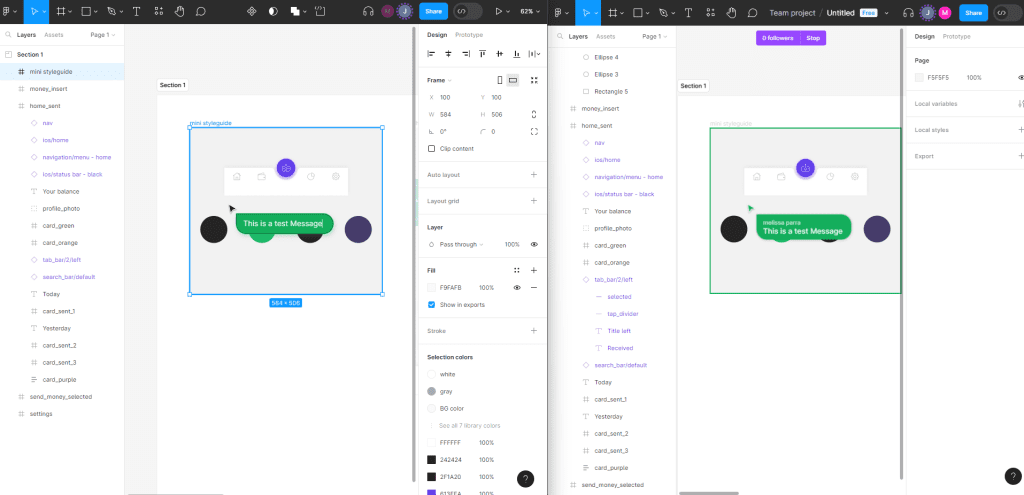
\includegraphics[width=0.8\textwidth]{figma.png}
	\caption{Alat za kolaboraciju Figma}
	
\end{figure}
    
\paragraph{Notion}  
je platforma za beleške i upravljanje projektima koja se koristi za kolaboraciju u realnom vremenu. Korisnici mogu da kreiraju i uređuju stranice, dodaju zadatke, tabele i baze podataka, dok istovremeno više korisnika može da pristupa i uređuje iste sadržaje.
    
\paragraph{Overleaf}  
je web-bazirana LaTeX platforma koja omogućava kolaborativno uređivanje tehničkih dokumenata, akademskih radova, i istraživačkih radova. Idealna je za naučne i tehničke projekte, gde više korisnika simultano piše i uređuje dokumente u LaTeX-u, s momentalnim prikazom rezultata. Pomoću Overleaf-a je napisan i ovaj diplomski rad.
    
Ovi alati predstavljaju ključne primere kako moderni editori omogućavaju bržu i efikasniju kolaboraciju, smanjujući potrebu za ručnom sinhronizacijom i olakšavajući zajednički rad na projektima.


\startnewsection
    
\section{Tehnike i Algoritmi za Sinhronizaciju i Rešavanje Konflikata u Višekorisničkim Editorima}

Fokusiraćemo se na tehnike i algoritme kod sinhronog kolaborativnog uređivanja dokumenata. 

\subsection{Mehanizam zaključavanja}

Kad god pričamo o deljenim resursima, prva stvar koja pada na pamet su \textbf{zaključavanja}.

Postoje dva učestala tipa zaključavanja.

\subsubsection{Pesimističko zaključavanje}

Pesimističko zaključavanje omogućava ekskluzivan pristup podacima od jedne strane, dok su sve ostale strane na čekanju. Često se koristi u situacijama gde je visoka verovatnoća konflikata, npr. u bankarskim sistemima, gde je važna tačnost podataka. Takođe, nema potrebe za razrešenjem konflikata, što čini ovaj pristup jednostavnijim. Zbog prirode rešenja, ovaj mehanizam može izazvati sporiji rad sistema.\cite{acharya2020}

\begin{figure}[h]
	\centering
	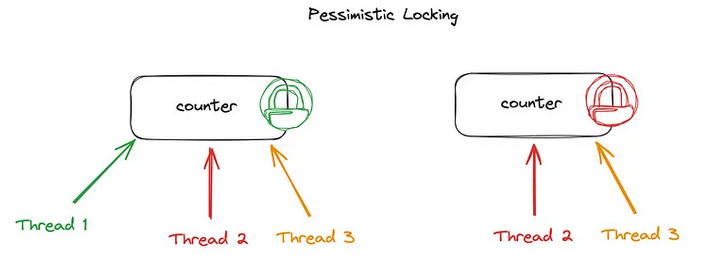
\includegraphics[width=0.8\textwidth]{pesimistic locking.png}
	\caption{Pesimističko zaključavanje}
	
\end{figure}

\subsubsection{Optimističko zaključavanje}

Optimističko zaključavanje je tehnika u upravljanju višekorisničkim pristupom koja se koristi za kontrolu pristupa deljenim resursima sa pretpostavkom da konflikti neće biti česti. Ova metoda omogućava korisnicima da slobodno pristupaju i uređuju resurse, a konflikti se rešavaju samo kada dođe do neslaganja prilikom ažuriranja resursa.\cite{acharya2020}

\begin{figure}[h]
	\centering
	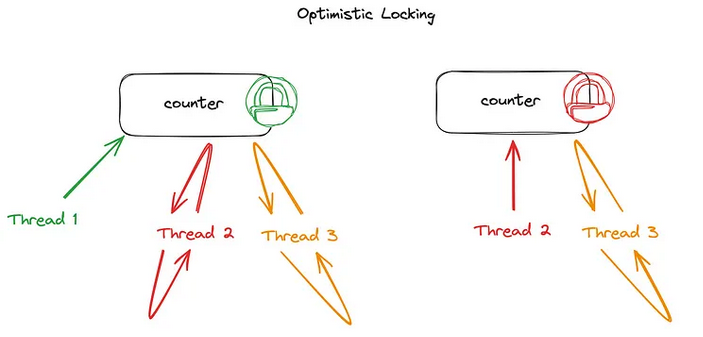
\includegraphics[width=0.8\textwidth]{optimistic locking.png}
	\caption{Optimističko zaključavanje}
	
\end{figure}

\paragraph{}
Problem sinhronizacije u višekorisničkim editorima \textbf{ne može da se reši pesimističkim zaključavanjem}. To je zato što bi u jednom trenutku samo jedan korisnik imao pristup menjanju podataka. Ovo bi bila izuetno spora kolaboracija. U optimističkom zaključavanju svi korisnici mogu da menjaju dokument u istom trenutku. Treba da uspostavimo pravila koja će razrešavati potencijalne konflikte.

Svaki deljeni resurs na serveru ima verziju, vremensku oznaku ili heš koji je povezan s njim. Kada klijent pročita podatke sa servera, pamti verziju povezanu s tim podacima. Zatim te podatke obrađuje lokalno. Kada želi da upiše nove podatke nazad na server, trebalo bi da poveća verziju. Sada, ako je u međuvremenu neki drugi klijent ažurirao podatke i verziju, prvi klijent \textbf{ne može} da upiše svoje podatke nazad jer njegova lokalna kopija nije nastala na osnovu te verzije sa servera. U tom slučaju se razrešavaju konflikti. Nekada klijent odbaci svoje lokalne promene, ponovo preuzme nove podatke sa servera i započne operaciju iznova. Dva najučestalija mehanizma koja razrešavaju konflikte su:

\begin{itemize}
	\item \textbf{Operational Transformation (OT)} \\
	      Algoritam koji omogućava automatsko upravljanje i sinhronizaciju promena u realnom vremenu. OT transformiše operacije uređivanja na način koji održava konzistentnost dokumenata između svih klijenata.
	              
	\item \textbf{Conflict-free Replicated Data Types (CRDT)} \\
	      CRDT koristi matematičke strukture koje omogućavaju da se promene automatski sinhronizuju među klijentima bez potrebe za centralizovanim serverom ili manuelnim razrešavanjem konflikata.
	              
	\item \textbf{Last-Writer-Wins (LWW)} \\
	      Ovaj jednostavan algoritam rešava konflikte tako što uzima poslednju izmenu koja je stigla na server kao važeću, bez obzira na to koja je starija verzija dokumenta.
	              
	\item \textbf{Version Control with Merging} \\
	      Verziona kontrola sa spajanjem koristi princip da klijenti rade na sopstvenim verzijama dokumenta, a zatim sistem pokušava automatski da spoji promene kada se one pošalju na server.
	      
\end{itemize}

OT i CRDT su najučestaliji algoritmi za automatsko razrešavanje konflikata, pa ćemo detaljno proći kroz ova dva pristupa.

\subsection{Operational Transformation(OT)}

\subsubsection{Prve verzije Google Docs-a}

Prve verzije Google Docs-a su koristile poređenje verzija dokumenata. Zamislimo da imamo dva klijenta, Anu i Branka, koji imaju sinhronizovane dokumente. Kad server primi promene od Ane, tada računa razliku verzija između nje i sebe i pokušava da ih spoji. Tada server šalje spojenu verziju Branku. Ako Branko ima svoje neposlate promene on pokušava da spoji primljenu serversku verziju sa svojom. Proces se ponavlja.

Često ovaj pristup ne daje dobre rezultate. Uzmimo sledeći primer:

\begin{figure}[h]
	\centering
	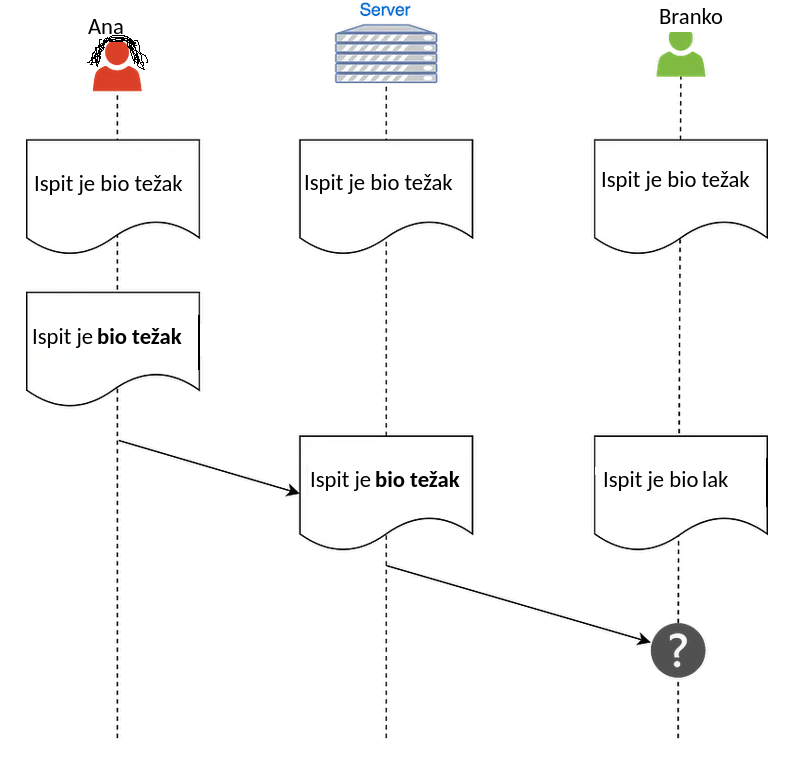
\includegraphics[width=0.8\textwidth]{ana i branko.png}
	\caption{Primer konflikta}
	
\end{figure}

Ana i Branko oboje počinju sa rečenicom "Ispit je bio težak". Ana podebljava reči "bio težak", a u isto vreme Branko menja reč "lak" u "težak". Anina verzija prva stiže do servera, primenjuju se promene i sada ta verzija stiže do Branka. Tačno rešenje treba da bude "Ispit je \textbf{bio lak}". Međutim, algoritam nema dovoljno informacija da izvrši tačno spajanje. Nešto od sledećeg bi takođe moglo da bude tačno rešenje: "Ispit je \textbf{bio težak} lak", "Ispit je bio \textbf{težak} lak", "Ispit je  \textbf{bio} lak \textbf{težak}".

\subsubsection{Novije verzije Google Docs-a}

Dokument se čuva kao niz operacija, i one se primenjuju redom, umesto poređenja verzija dokumenata. Sada treba razumeti \textbf{kada} se primenjuju promene, kolaboracioni protokol. U Google Docs-u postoje tri različita tipa promena:

\begin{itemize}
	\item Ubacivanje teksta
	\item Brisanje teksta
	\item Primena stila
\end{itemize}

Kada se uređuje dokument, sve izmene se dodaju u zapis promena kao jedna od ove tri vrste, i zapis promena se ponovo izvršava od određene tačke kada se otvori dokument.

Uzmimo sledeći primer:

Ana i Branko kreću od dokumenta "LIFE 2017". Ana menja 2017 u 2018 i zapisuju se dve operacije:

\begin{figure}[H]
	\centering
	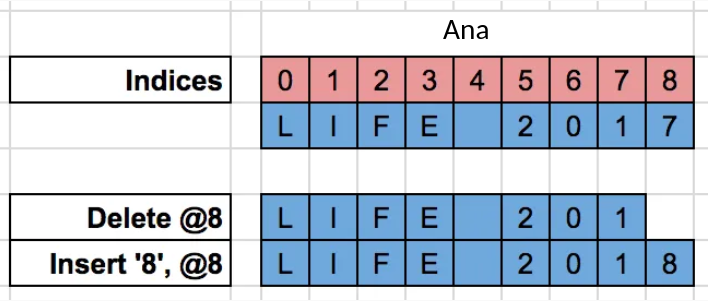
\includegraphics[width=0.8\textwidth]{primer31.png}
	\caption{Ana primenjuje dve operacije}
	
\end{figure}

U isto vreme Branko menja tekst u "CRAZY LIFE 2017":

\begin{figure}[H]
	\centering
	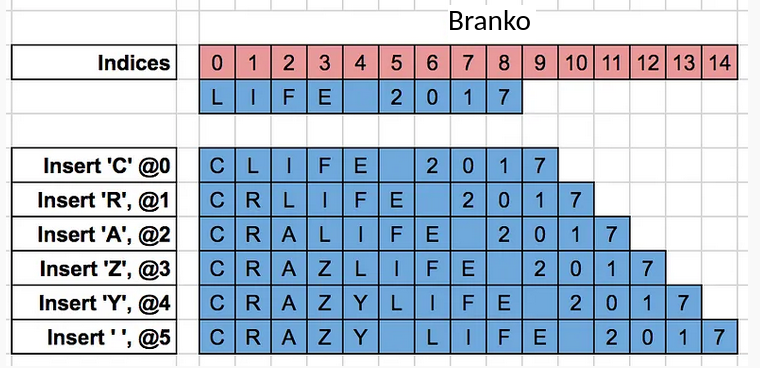
\includegraphics[width=0.8\textwidth]{primer32.png}
	\caption{Branko primenjuje svoje operacije}
	
\end{figure}

Ako bi Branko samo primenio Aninu operaciju brisanja kada je primio, onda bi dobio nevalidan dokument(cifra 7 je trebalo da bude obrisana). 

\begin{figure}[H]
	\centering
	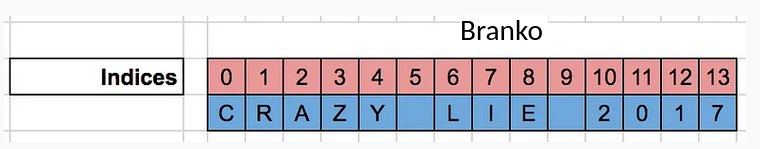
\includegraphics[width=0.8\textwidth]{primerlosbranko.png}
	\caption{Loša primena operacija}
	
\end{figure}

Branko treba da prilagodi operaciju brisanja u skladu sa svojim lokalnim izmenama kako bi dobio ispravno stanje dokumenta:

\begin{figure}[H]
	\centering
	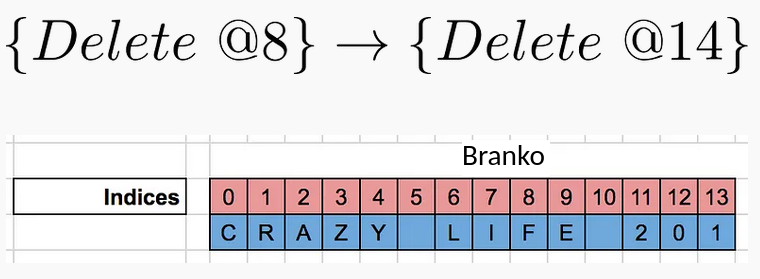
\includegraphics[height=4cm]{primer33.png}
	\caption{Dobra primena operacija}
	
\end{figure}

Formalnije, pogledajmo sledeći primer:

\begin{figure}[H]
	\centering
	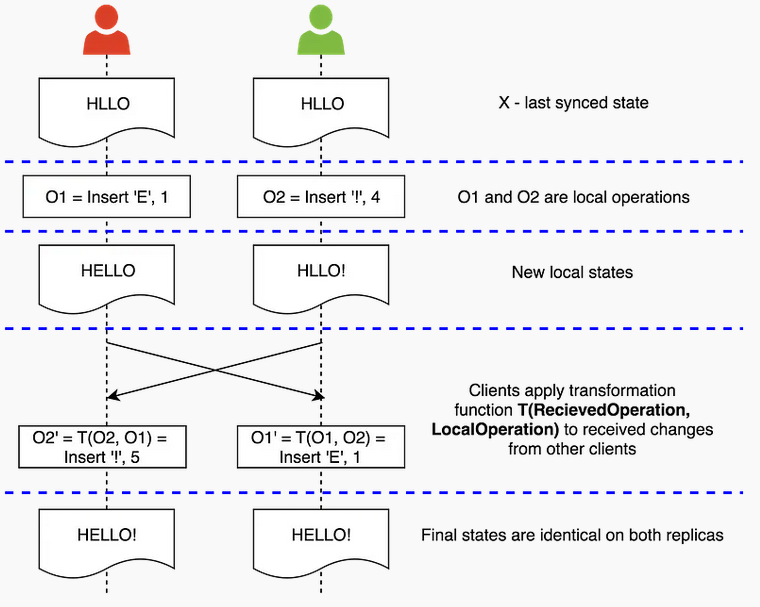
\includegraphics[width=0.8\textwidth]{formalniprimer.png}
	\caption{Formalni primer}
	
\end{figure}

onda važi da je:

\[
	\huge
	E = O1'(O2(X)) = O2'(O1(X))
\]

Upravo smo opisali kako funkcioniše algoritam OT.

\subsubsection{Modeli konzistentnosti(CCI model)}

Modeli konzistentnosti odnose se na pravila koja definišu kako se više kopija podataka sinhronizuju u distribuiranim sistemima. Nekoliko modela konzistentnosti je kreirano da pruži konsistentnost za OT.

\paragraph{CCI Model}

\begin{itemize}
	\item \textbf{Konvergencija} \\
	      Sve replike istog dokumenta moraju biti identične nakon primene svih operacija.
	      
	      \begin{figure}[H]
	      	\centering
	      	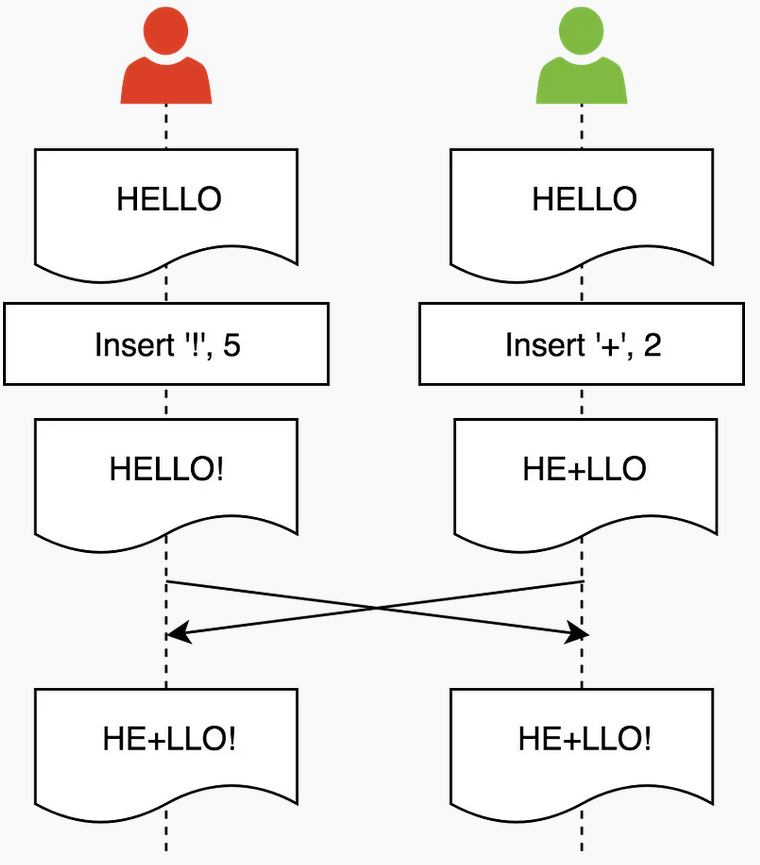
\includegraphics[height=7cm]{CCImodel.png}
	      	\caption{CCI model}
	      	
	      \end{figure}
	      Ana i Branko počinju od istog dokumenta, onda rade lokalne primene i replike divergiraju(ovim dobijamo dobru responzivnost). Svojstvo konvergencije zahteva do klijenti vide isti dokument nakon primenjenih operacija koje su dobili.
	      
	\item \textbf{Očuvanje namere} \\
	      Osigurava da će efekat izvršavanja operacije na bilo kom stanju dokumenta biti isti kao namera operacije. Namera operacije se definiše kao efekat njenog izvršenja na repliku na kojoj je kreirana. Razmotrimo primer u kojem je ovo svojstvo narušeno:
	      
	      \begin{figure}[H]
	      	\centering
	      	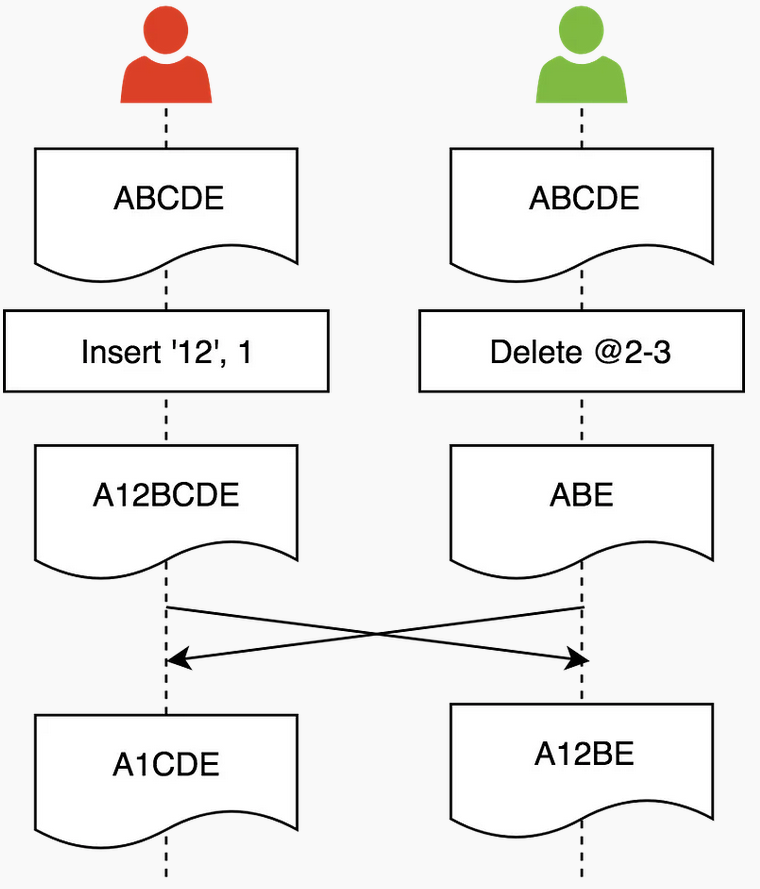
\includegraphics[height=7cm]{OcuvanjeNamere.png}
	      	\caption{(Ne)Očuvanje namere}
	      	
	      \end{figure}
	      Ana i Branko počinju od istog stanja dokumenta, zatim vrše svoje lokalne izmene. Namera Anine operacije je da ubaci '12' na poziciju 1, dok je namera Brankove operacije da obriše 'CD'. Nakon sinhronizacije, Bobova namera je narušena. Iako su replike različite, to nije neophodno za svojstvo očuvanja namere. 
	      
	\item \textbf{Očuvanje kauzalnosti} \\
	      Operacije moraju biti izvršene u skladu sa njihovim prirodnim redosledom uzroka i posledica tokom procesa kolaboracije (zasnovano na relaciji "dogodilo se pre"). Pogledaemo primer gde je kauzalnost naruena:
	      
	      \begin{figure}[H]
	      	\centering
	      	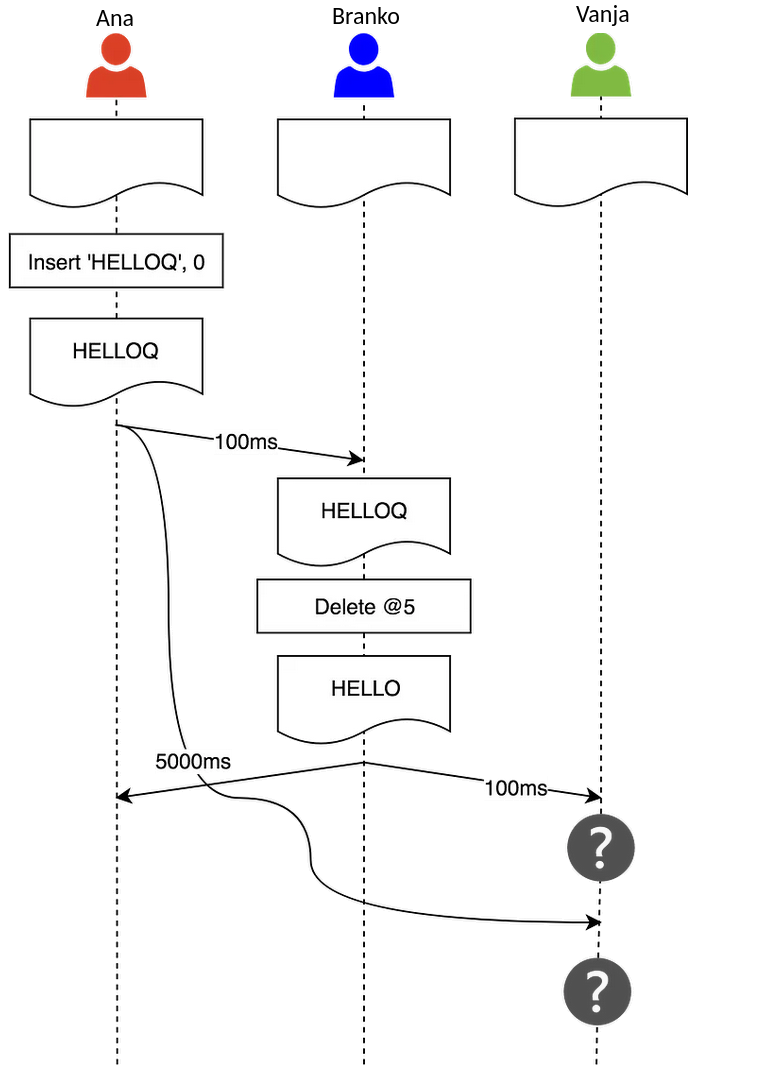
\includegraphics[height=10cm]{nepostovanjeKauzalnosti.png}
	      	\caption{Nepoštovanje kauzalnosti}
	      	
	      \end{figure}
	      
	      Ana, Branko i vanja kreću od istog stanja dokumenta. Ana pravi promenu i šalje drugim klijentima. Branko prima prvi promenu, menja pravopisnu grešku i šalje promene ostalim klijentima. Zbog zagušenja u mreži, Vanja prvo dobija Brankovu operaciju, koja je brisanjew simbola koji još uvek ne postoji u njegovoj replici.
	      
	      Operational Transformation ne može da obezbedi ovo svojstvo, pa se mogu koristiti drugi algoritmi kao što je Vektorski sat.
	      
	      \textbf{Vektorski sat} je struktura podataka koja se koristi za određivanje delimičnog redosleda događaja u distribuiranom sistemu i otkrivanje kršenja uzročnosti. Poruke između procesa sadrže stanje logičkog sata procesa koji šalje poruku. Vektorski sat u sistemu sa N procesa je niz od N logičkih satova, gde svaki proces ima po jedan sat. Svaki proces lokalno čuva kopiju tog niza sa najvećim mogućim vrednostima, što predstavlja stanje globalnog sata.
	      
	      \begin{enumerate}
	      	\item Inicijalno svi satovi imaju vrednost \textbf{nula}.
	      	\item Pre pravljenja operacije, proces \textit{i} inkrementira \textit{i}-ti element svog vektorskog sata za 1.
	      	      \[ VC_i = VC_i + 1 \]
	      	\item Svaki put kada proces šalje poruku, inkrementira sopstveni logički sat u vektoru za 1, zatim šalje ceo vektor.
	      	\item Svaki put kada proces \textit{i} prima poruku, inkrementira \textit{i}-ti element svog vektorskog sata za 1. Za sve ostale procese, uzima maksimum odgovarajućeg elementa u poruci i svoje lokalne vrednosti u vektoru.
	      	      \[ VC_j = max(Vmsg_j, VC_j)\]
	      	      \begin{figure}[H]
	      	      	\centering
	      	      	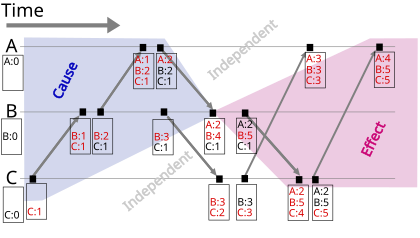
\includegraphics[height=5cm]{vektorskisat.png}
	      	      	\caption{Vektorski sat}
	      	      	
	      	      \end{figure}
	      	                  
	      \end{enumerate}
	      
\end{itemize}

\subsubsection{Kritike}

\begin{itemize}
	\item Sve promene u dokumentu moraju biti sačuvane u nizu operacija
	\item Implementacija OT-a može biti veoma kompleksan zadatak, citat sa Vikipedije:
	      
	      \begin{quote}
	      	Nažalost, implementacija OT-a je užasna. Postoji milion algoritama sa različitim kompromisima, uglavnom zarobljenih u akademskim radovima. Algoritmi su zaista teški i vremenski zahtevni za pravilnu implementaciju. [...] Wave je trajao 2 godine da se napiše, a ako bismo ga danas ponovo pisali, trajalo bi skoro isto toliko dugo. 
	      	\begin{flushright}
	      		--- Joseph Gentle, bivši inženjer Google Wave-a i autor Share.JS biblioteke
	      	\end{flushright}
	      \end{quote}
	              
\end{itemize}

\subsection{Conflict-free Replicated Data Types(CRDT)}

Koristili smo aplikacije kao što je Google Drive. On omogućava:

\begin{itemize}
	\item Rad u Offline režimu
	\item Pristup sa više različitih uređaja
	\item Više ljudi koji istovremeno uređuju iste podatke
\end{itemize}

Zadatak koji programeri tih sistema moraju rešiti je kako osigurati "glatku" sinhronizaciju podataka u takvim situacijama. U idealnom slučaju, interakcija korisnika ne bi trebalo da bude potrebna.

Kao i OT, CRDT takođe automatski razrešava konflikte prilikom spavanja, tako što uvodi poseban skup osnovnih tipova podataka.

\subsubsection{Snažna eventualna konzistentnost}

Kada se priča o konzistentnosti, spominju se ova tri termina:

\begin{itemize}
	\item \textbf{Snažna konzistentnost(SC)}: sve operacije pisanja su izvršene striktno sekvencijalno, a operacije čitanja sa replika vraćaju isti, poslednje napisan rezultat. Konsenzus u realnom vremenu je potreban da bi se rešili konflikti, omogućava da do n/2-1 čvorova bude van funkcije.
	\item \textbf{Eventualna konzistentnost(EC)}: promene se prvo izvrše lokalno, a zatim se propagiraju. Čitanje na nekim replikama može vratiti zastarelo stanje. U slučaju konflikata, potrebno je odlučiti šta je ispravno stanje. To znači da je konsenzus i dalje potreban, ali ne u realnom vremenu.
	\item \textbf{Snažna eventualna konzistentnost(SEC)}: EC + replike imaju mehanizam sa automatski rešavaju konflikte, tako da konsenzus nije potreban. Dozvoljava da n-1 čvorova bude van funkcije.
\end{itemize}

Postoji dosta istraživanja koja se bave eventualnom konzistentnošću. Istražuju se druge varijante koje nisu toliko ograničavajuće poput SC. CRDT pruža \textbf{snažnu eventualnu konzistentnost}.

\subsubsection{"Likes and hits" problem}

"Likes and hits" problem je dugo poznati izazov u distribuiranim sistemima, konkretno kod društvenih mreža, gde korisnici mogu da interaguju sa sadržajem u realnom vremeenu(lajkovanjem postova ili videa, ili povećavajući gledanost). Suština problema je održavanje preciznog broja lajkova, gledanja, ili drugih metrika kroz distribuirani sistem gde se sadržajem može interagovati sa različitih lokacija.

\paragraph{Broj pogodaka na google.com:}

Google.com prima oko 150000 zahteva po sekundi sa različitih delova planete. Očigledno je da će se brojač ažurirati asinhrono. Možemo da uvedemo redove koji izvršavaju zadatke asinhrono, ali ako dobijemo zahtev za vrednost brojača moramo da izvršimo replikaciju, inače nam mnogo zahteva za čitanje može oboriti server.

Da li možemo da zaobiđemo redove ako već radimo replikaciju?

\begin{figure}[H]
	\centering
	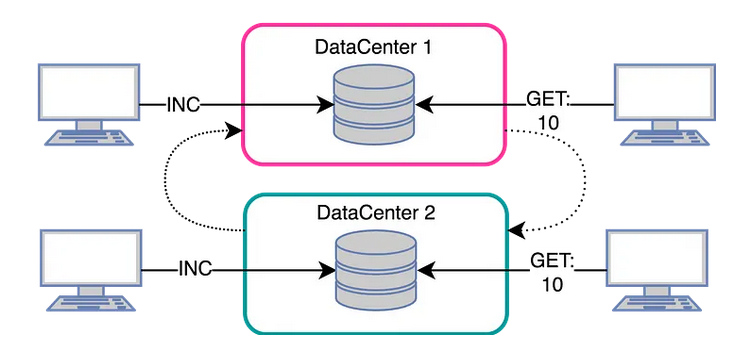
\includegraphics[height=5cm]{replikacija.png}
	\caption{Replikacija}
	
\end{figure}
    
\subsubsection{Tipovi u CRDT-u, semantika razrešavanja konflikata}

CRDT-ovi su specijalni tipovi podataka koji konvergiraju podatke sa svih replika baze podataka. Popularni CRDT-ovi su G-brojači (brojači koji samo rastu), PN-brojači (pozitivno-negativni brojači), registri, G-skupovi (skupovi koji samo rastu), 2P-skupovi (dvostepeni skupovi), OR-skupovi (skupovi sa zapaženim uklanjanjem), itd. Iza kulisa, oni se oslanjaju na sledeće matematičke osobine da bi konvergirali podatke:

\begin{itemize}
	\item \textbf{Komutativnost}: $a \circ b = b \circ a $
	\item \textbf{Asocijativnost}: $a \circ (b \circ c) = (a \circ b) \circ c $
	\item \textbf{Idempotentnost}: $a \circ a = a $
\end{itemize}
    
G-brojač je primer operativnog CRDT-a koji spaja operacije. Ovde, a + b = b + a i a + (b + c) = (a + b) + c. Replike međusobno razmenjuju samo ažuriranja (sabiranja). CRDT spaja ažuriranja dodavanjem. G-skup, na primer, primenjuje idempotentnost ({a, b, c} U {c} = {a, b, c}) kako bi spojio sve elemente. Idempotentnost izbegava dupliranje elemenata dodanih u strukturu podataka dok putuju i konvergiraju kroz različite putanje.

\paragraph{Strukture podataka bez konflikata: G-brojači, PN-brojači, G-skupovi:}

Svi ovi tipovi podataka su dizajnirani tako da ne dolazi do konflikata. Tabele ispod prikazuju kako se podaci sinhronizuju između replika baza podataka. 

\begin{figure}[H]
	\centering
	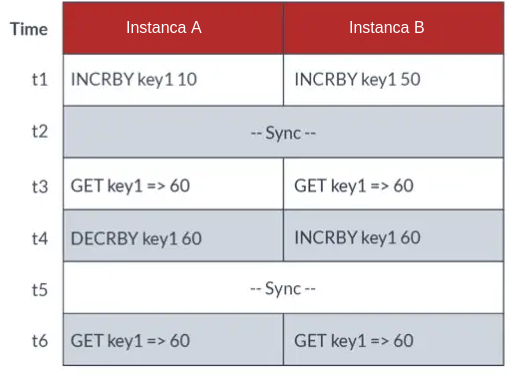
\includegraphics[height=5cm]{crdt1.png}
	\caption{Primer kako PN-brojači sinhronizuju promene}
	
\end{figure}

\begin{figure}[H]
	\centering
	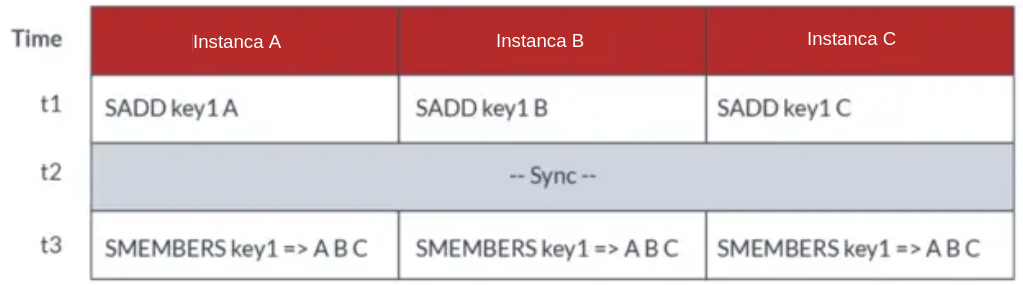
\includegraphics[width=12cm]{crdt2.png}
	\caption{G-skupovi garantuju unikatne elemente}
	
\end{figure}

G-brojači i PN-brojači su popularni za primene kao što su globalno glasanje, brojanje strimova, praćenje aktivnosti i slično. G-skupovi se često koriste za implementaciju blokčejn tehnologije. Na primer, Bitkoin koristi zapise u blokčejnu koji se samo dodaju.

\paragraph{Strukture podataka sa konfliktima}:

\textbf{Registri} prirodno dolaze sa konfliktima. Obično koriste tehnike kao što su "Last Write Wins" (LWW) ili rešavanje konflikata zasnovano na kvorumu. Na slici ispod prikazan je primer kako registar rešava konflikt prateći LWW politiku.

\begin{figure}[H]
	\centering
	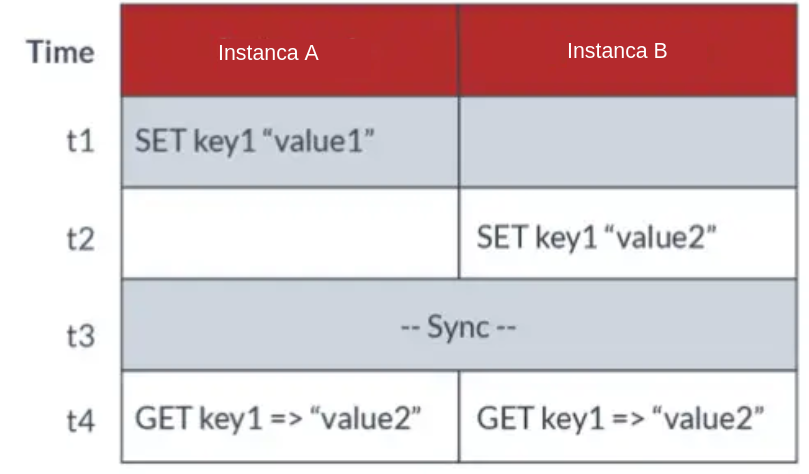
\includegraphics[width=10cm]{crdt3.png}
	\caption{LWW pristup kod registara}
	
\end{figure}

\textbf{2P-skupovi(two phase sets)} održavaju dva skupa G-setova — jedan za dodate stavke i drugi za uklonjene stavke. Replike razmenjuju dodatke G-setova prilikom sinhronizacije. Konflikt nastaje kada se isti element nađe u oba skupa. U nekim CRDT bazama podataka, to se rešava politikom „Dodavanje pobeđuje brisanje”.

\begin{figure}[H]
	\centering
	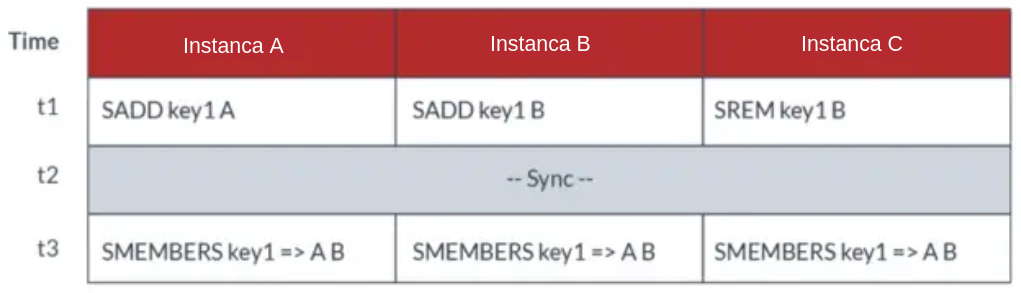
\includegraphics[width=12cm]{crdt4.png}
	\caption{"Dodavanje pobeđuje brisanje" za 2P-skupove}
	
\end{figure}

\subsubsection{"Likes and hits" rešenje}

U kontekstu problema sa "Likes" i "Hits", CRDT-ovi poput PN-brojača nude rešenje za sinhronizaciju velikih količina podataka koji se brzo menjaju i pristupaju sa različitih mesta. Iako rezultati mogu biti zastareli dok sinhronizacija ne bude obavljena, krajnji cilj je da se obezbedi eventualna konzistentnost između svih replika bez potrebe za stalnim sinhronizovanjem pri svakom zahtevu. Nakon završene sinhronizacije, sve replike će konvergirati na istu finalnu vrednost.

\begin{figure}[h]
	\centering
	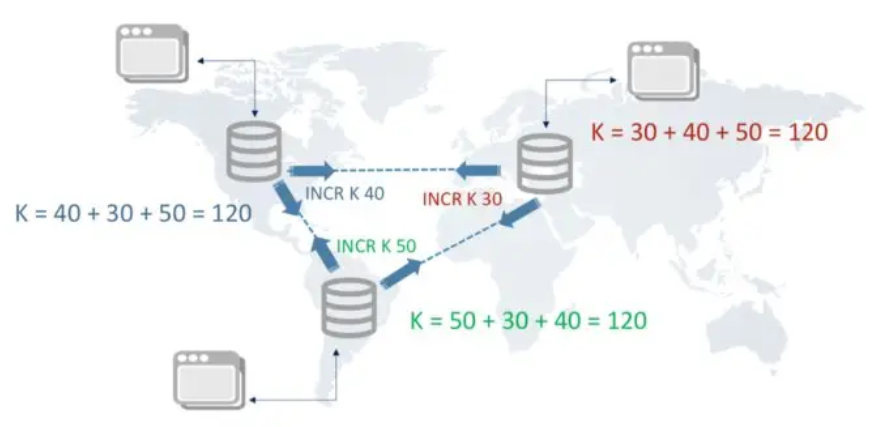
\includegraphics[width=12cm]{likes and hits.png}
	
\end{figure}

\startnewsection

\section{Implementacija kolaborativnog editora}

\subsection{Motivacija}

\subsubsection{FAANG intervjui}

FAANG\footnote{Facebook, Amazon, Apple, Netflix, Google} intervjui je termin za standardizovane intervjue koje sprovode velike korporacije. Najčešći oblici intervjua su:

\begin{itemize}
    \item \textbf{Algoritamski intervju} Kandidat dobije algoritamski zadatak za koji treba da smisli optimalno rešenje. Zajedno sa intervjuerom idejno smišlja algoritam, i na kraju taj algoritam implementira. Ponekad se pokreću testovi da se proveri da li algoritam dobro radi.

    \item \textbf{Intervju za dizajn sistema} Kandidat dobije zadatak da osmisli kako bi dizajnirao zadat sistem. Kroz pitanja koja su upućena interjvueru dolazi do potrebnih informacija, formira skup zahteva sistema, i opisuje komponente i njihovu vezu. Ponekad se od njega traži da detaljnije objasni neke delove sistema. Ponekad se traži pseudokod za neku komponentu sistema.
\end{itemize}

Okruženje u kom se sprovode ovi intervjui podrazumevaju alat koji služi za kolaboraciju, u kom kandidat može da piše i pokreće svoj kod, a gde intervjuer može da ostavlja komentare ili koriguje neki deo koda kandidata(lepi test primere, tekst zadatka itd.). Upravo je ovo motivacija za implementaciju kolaborativnog editora, pravljenje okruženja pomoću kod se mogu izvoditi intervjui, ili spremanje za intervju(Mock intervjui\footnote{Mock intervju su simulacije stvarnih intervjua koje pomažu kandidatima da vežbaju i dobiju povratne informacije kako bi se bolje pripremili za pravi intervju.}).


\subsection{Arhitektura}

Za komunikaciju klijenata, trebaće nam jedan \textbf{Node.js} server, kroz koji će klijenti komunicirati. Na serveru ćemo čuvati i podatke o sesiji, zadatke, proteklo vreme, kao i modul koji čuva podatke i komunicira sa konfliktima pomoću biblioteke \textbf{share-db}. \href{https://share.github.io/sharedb/}{Share-db} je biblioteka koja omogućava saradnju u realnom vremenu u aplikacijama koristeći mehanizam za sinhronizaciju podataka između više korisnika. \cite{sharedb}

Klijentska strana će biti implementiran u React-u, iz više razloga. Prvi je zato što će nam trebati share-db klijent, koji komunicira sa serverom, i šalje operacije u standardizovanom formatu. Drugi je zato što ćemo koristiti \href{https://microsoft.github.io/monaco-editor/}{Monaco Editor}, open source editor koji nudi razne standardne funkcionalnosti modernog editora, kao što je automatsko dovršavanje reči, prikaz više kursora istovremeno, automatsko formatiranje koda itd. Na klijentu ćemo vršiti komunikaciju sa serverom preko soketa\footnote{Soket je krajnja tačka za komunikaciju između dva računara ili procesa preko mreže, koja omogućava slanje i primanje podataka.}. Pored stvari vezanih za multi kolaborativan editor, imaćemo i druge elemente koje su potrebne za alat pomoću kog može da se sprovodi intervju(video komunikacija, pokretanje koda, algoritam za dodelu zadatka itd.) koje nećemo detaljno objašnjavati.

\begin{figure}[H]
	\centering
	\includegraphics[width=15cm]{editor.jpeg}
	
\end{figure}
SLIKA ARHITEKTURA

\subsection{Implementacija}

\subsubsection{Inicijalizacija sesije}

Na serverskoj strani inicijalizujemo objekat share, koji nam treba za prihvatanje konekcija sa klijenta:

\begin{mylisting}[label={lst:example}]{Inicijalizacija servera}
\begin{lstlisting}
var express = require('express')
var WebSocket = require('ws')
var http = require('http')
var ShareDB = require('sharedb')
var WebSocketJSONStream = require('@teamwork/websocket-json-stream')

var app = express()
var server = http.createServer(app)
var webSocketServer = new WebSocket.Server({server: server})

const share = new shareDB({ presence: true });
webSocketServer.on('connection', (webSocket) => {
  var stream = new WebSocketJSONStream(webSocket)
  share.listen(stream)
})

server.listen(8080)
\end{lstlisting}
\end{mylisting}


Definisaćemo i objekat connection
\begin{mylisting}[label={lst:example}]{Connection objekat}
\begin{lstlisting}
const connection = share.connect();
\end{lstlisting}
\end{mylisting}

Pomoću ovog objekta imamo pristup \textit{in-memory} bazi od share-db-a, i prilikom klijentskog zahteva možemo vratiti odgovarajući dokument od sesije:

\begin{mylisting}[label={lst:example}]{Primanje zahteva}
\begin{lstlisting}
app.post("/", (req, res) => {
  let sessionId = req.body.sessionId;
  
  const doc = connection.get("session", sessionId);
  doc.fetch((err) => {
    if (err) throw err;

    if (doc.type == null) {
      doc.create(initialDoc);
    }
  });

  //fetches task for the sessionId
  fetchTaskData(sessionId)
    .then((data) => res.json(data));
}
  
\end{lstlisting}
\end{mylisting}

Kod kreiranja dokumenta možemo staviti odgovarajući \textit{json} objekat, recimo inicijalni kod. 

\begin{mylisting}[label={lst:example}]{Inicijalni dokument}
\begin{lstlisting}
const initialDoc = {
    sourceCode : {
        "#include <iostream>
        int main() {
            return 0;
        }"
    },
    lang: "c++"
};
\end{lstlisting}
\end{mylisting}

Na klijentskoj strani, pri inicijalizaciji editor komponente ćemo uspostaviti vezu sa serverom:

\begin{mylisting}[label={lst:example}]{main.tsx}
\begin{lstlisting}
"use client";
...
import shareDB from "sharedb/lib/client";

const Editor: React.FC = () => {
  useEffect(() => {
    let rws = new ReconnectingWebSocket(ws_url);
    rws.addEventListener("open", () => {
      let connection = new shareDB.Connection(rws);
      let doc = connection.get("session", startInfo.sessionId);
    }
  }, []);
}
\end{lstlisting}
\end{mylisting}

Koristićemo \textit{monaco} editor\cite{monacoeditor}:

\begin{mylisting}[label={lst:example}]{monacoEditor.tsx}
\begin{lstlisting}
import { MonacoProps } from "@/app/editor/types/types";
import Editor from "@monaco-editor/react";

const MonacoEditor = (props: MonacoProps) => {
  const { language, code, readOnly, editorDidMount, editorOnChange } = props;

  return (
    <Editor
      options={options}
      language={language}
      value={code}
      onMount={editorDidMount}
      onChange={editorOnChange}
    />
  );
};
export default MonacoEditor;
\end{lstlisting}
\end{mylisting}

\subsubsection{Detektovanje promena i slanje operacija}

Na svaku promenu stanja kod klijenta koje može biti:

\begin{itemize}
    \item Dodavanje karaktera
    \item Brisanje karaktera
    \item Promena kursora
    \item Promena jezika
\end{itemize}

treba izvršiti operaciju, a zatim je i emitovati ka drugom klijentu.


\begin{mylisting}[label={lst:example}]{main.tsx}
\begin{lstlisting}
doc.subscribe(err => {
  if (err) throw err;
  const presence = connection.getPresence("session");
  presence.subscribe(err => {
    if (err) throw err;
  });
  let localPresenceInstance = presence.create();
  const newBinding = initializeBinding([doc, monaco, code, lang]);
  newBinding.setup();
});
\end{lstlisting}
\end{mylisting}

U \textit{listener}-u monaco editora ćemo pozvati metodu koja pravi novu operaciju:

\begin{mylisting}[label={lst:example}]{Monaco Listener}
\begin{lstlisting}
const editorOnChange = (newValue: any, e: any) => {
  binding.inputListener(newValue, e);
};
\end{lstlisting}
\end{mylisting}

Metoda \textit{inputListener} beleži promene, registruje koji tekst se promenio i na kojoj poziciji, i prema tome zove operacije \textit{insert} ili \textit{remove}. 

\begin{mylisting}[label={lst:example}]{textBinding.tsx}
\begin{lstlisting}
const inputListener = (newValue: any, e: any) => {
  let previous = this.doc.data[this.path[0]];
  let value = newValue;
  if (previous === value) return;

  let start = 0;
  let end = 0;
  while (previous.charAt(start) === value.charAt(start)) {
    start++;
  }
  while (
    previous.charAt(previous.length - 1 - end) === 
    value.charAt(value.length - 1 - end) &&
    end + start < previous.length &&
    end + start < value.length
  ) {
    end++;
  }
  if (previous.length !== start + end) {
    let removed = previous.slice(start, previous.length - end);
    remove(start, removed, e.changes[0].rangeOffset);
  }
  if (value.length !== start + end) {
    let inserted = value.slice(start, value.length - end);
    insert(start, inserted, e.changes[0].rangeOffset);
  }
};
\end{lstlisting}
\end{mylisting}

Slede i \textit{insert} i \textit{remove} funkcije:

\begin{mylisting}[label={lst:example}]{\textit{insert} i \textit{remove}}
\begin{lstlisting}

insert = (index: any, text: any, rangeOffset: number) => {
  let path = this.path.concat(index);
  let op = { p: path, si: text, rangeOffset: rangeOffset };
  this.doc.submitOp(op);
};

remove = (index: any, text: any, rangeOffset: number) => {
  let path = this.path.concat(index);
  let op = { p: path, sd: text, rangeOffset: rangeOffset };
  this.doc.submitOp(op);
};
\end{lstlisting}
\end{mylisting}

Objekat \textit{doc} ima ugrađenu funkciju submitOp koja operaciju šalje na server, drugom klijentu šalje promene.

Takođe, želimo da našu trenutnu poziciju kursora propagiramo do drugog klijenta:

\begin{mylisting}[label={lst:example}]{Propagiranje pozicije kursora do drugog klijenta}
\begin{lstlisting}
monaco.onDidChangeCursorSelection((e: any) => {
  binding.localPresence.submit(e.selection, (err: Error) => {
    if (err) throw err;
  });
});
\end{lstlisting}
\end{mylisting}

\subsubsection{Primena promena od drugog klijenta}

Objekat \textit{presence} koji smo dobili od konekcije pri početku sesije, ima mogućnost osluškivanja promena sa servera:

\begin{mylisting}[label={lst:example}]{Propagiranje pozicije kursora do drugog klijenta}
\begin{lstlisting}
presence.on("receive", (id, range) => {
  let isPos = range.startLineNumber === range.endLineNumber &&
  range.startColumn === range.endColumn;
  const decorations = editor.deltaDecorations(binding.decorations, [
    {
      range: new monaco.Range(range.startLineNumber, 
      range.startColumn, range.endLineNumber, range.endColumn),
      options: {
        className: isPos ? "cursor-position" : "cursor-selection",
      },
    },
  ]);
  binding.updateDecorations(decorations);
  binding.updateRange(range);
});
\end{lstlisting}
\end{mylisting}

Operacije vezane za kod se automatski primenjuju, a samostalno implementiramo pomeranje kursora. Kod monaco editora prikaz kursora je zapravo prikaz selekcije koja počinje i završava se na istom karakteru. U zavisnosti od toga da li je selekcija dužine 0 ili veće, prikazujemo selekciju u stilu kursora ili selekcije.

\subsubsection{Završetak sesije}

Dodaćemo dugme na sredini stranice koje ima mogućnost prekida sesije. Treba zatvoriti \textit{socket}, prekinuti vezu sa \textit{doc i presence} objektima, prestati emitovanje preko \textit{localPresence} objekta, zatvoriti konekciju.

\begin{mylisting}[label={lst:example}]{main.tsx}
\begin{lstlisting}
const endSession = () => {
  rws.close();
  doc.unsubscribe();
  presence.unsubscribe();
  localPresence.destroy();
  connection.close();
};
\end{lstlisting}
\end{mylisting}

\startnewsection

\section{Postojeća rešenja}

\subsection{Etherpad}

Etherpad je \textit{open-source} alat za zajedničko uređivanje teksta u realnom vremenu, gde više ljudi može istovremeno raditi na istom dokumentu. Sve promene su odmah vidljive, a svaki korisnik ima svoju boju kako bi se lakše pratilo ko šta piše. Koristan je za timsku saradnju.\cite{etherpad}

\begin{figure}[H]
	\centering
	\includegraphics[width=12cm]{etherpad_screenshot.png}
	\caption{Etherpad}
	
\end{figure}

\subsubsection{Ideja}
Koristi OT kao algoritam za automatsko razrešavanje konflikata, sa malo drugačijim transformacionim funkcijama - šalje promene na server u sledećem obliku:

\[ (p1 -> p2)[c_1, c_2, …] \], gde je:

\begin{itemize}
    \item $p_1$ — dužina dokumenta pre izmene
    \item $p_2$ — dužina dokumenta nakon izmene
    \item $c_i$ — dve mogućnosti:
    \begin{itemize}
        \item ako je $c_i$ — broj ili opseg brojeva, to su indeksi nepromenjenih karaktera, ili
        \item ako je $c_i$ — karakter ili string, to znači ubacivanje novih elemenata u dokument
    \end{itemize}
\end{itemize}

Primer:

\begin{verbatim}
"" + (0 -> 5)["Hello"] = "Hello"
"Hllo World" + (10 -> 14)[0, 'e', 1–9, "!!!"] = "Hello World!!!"
\end{verbatim}

Dokument se formira kao hronološki niz takvih promena (changeset-ova) primenjenih na prazan dokument.

Možemo primetiti da server ne može jednostavno primeniti promene od klijenata jer dužine dokumenata mogu biti različite. Na primer, ako klijenti A i B počnu od istog dokumenta X dužine $n$ i izvrše sledeće promene respektivno:

\begin{align*}
A: & \quad (n \to n_a)[\dots], \\
B: & \quad (n \to n_b)[\dots]
\end{align*}

tada je $B(A(X))$ nemoguće jer B zahteva dokument dužine $n$, ali dokument ima dužinu $n_a$ nakon što je A primenjen. Da bi se rešio ovaj problem, Etherpad uvodi tzv. \emph{merge} funkciju koja uzima 2 changeset-a koja se odnose na istu verziju dokumenta i računa novi jedinstveni changeset. Potrebno je da:

\[ m(A,B) = m(B,A) \]

Nije od velike koristi računati $m(A, B)$ kada klijent A primi promene od klijenta B, jer $m(A, B)$ se odnosi na stanje $X$, ali A je u stanju $A(X)$. Umesto toga, treba izračunati $A'$ i $B'$ tako da:

\[ B'(A(X)) = A'(B(X)) = m(A,B)(X) \]

Radi jednostavnosti, definišimo funkciju \emph{follow} $f$:

\[ f(A,B) = B' \]
\[ f(B,A) = A' \]
\[ f(A,B)(A) = f(B,A)(A) = m(A,B) = m(B,A) \]

Primer:

\[ X = (0 \to 8)["baseball"] \]
\[ A = (8 \to 5)[0-1,"si",7] // == "basil"\]
\[ A = (8 \to 5)[0,"e",6,"ow"] // == "below"\]

Onda:

\[ A' = f(B,A) = (5 \to 6)[0,1,"si",3,4] \]
\[ B' = f(A,B) = (5 \to 6)[0,"e",2,3,"ow"]\]
\[ m(A,B) = m(B,A) = A(B') = B(A') = (8 \to 6)[0, "esiow"]\]

Dakle, uspeli smo da pomoću funkcije \textit{f} postignemo isto stanje dokumenta nakon primene operacija.

\subsubsection{Kritike}

Etherpad ima problem sa performansama kada korisnici uređuju vrlo velike dokumente, pogotov kada mnogo korisnika radi na istom dokumentu. Takođe je interfejs pomalo zastareo, podseća na Google Docs, ali sa manje funkcionalnosti. 

Okruženje je namenjeno kolaboraciji na dokumentima, ne koristi se toliko za kolaboraciju u pisanju koda, jer je editor tipičan tekstualni editor.

\subsection{Firepad}

Firepad je takođe \textit{open-source} alat za zajedničko uređivanje teksta u realnom vremenu. Pored tekstualnog, sadrži i kod editor, pa je pogodan i za pair-programming ili intervju sesije. Implementiran je od strane Firebase tima. \cite{firepad}

\subsubsection{Ideja}

Zanimljivost kod Firepad-a za razliku od drugih rešenja je što koristi Firebase za slanje operacija između klijenata. To znači da server nije potreban, jer se klijenti direktno povezuju i razmenjuju informacije preko Firebase-a. 

\paragraph{Firebase Realtime Database: } svaka izmena teksta se sinhronizuje putem Firebase baze podataka. Kada jedan korisnik napravi promenu, ona se odmah snima u bazu, a svi ostali korisnici automatski dobijaju tu izmenu zahvaljujući real-time sposobnostima Firebase-a.

\paragraph{Dokument u Realtime Database: } Firepad čuva dokumente kao JSON objekte u Firebase-u. Struktura može sadržavati tekstualne podatke, istoriju uređivanja i metapodatke kao što su korisnici koji trenutno uređuju dokument.

Firepad takođe koristi OT za rešavanje konflikata. Moguće je i offline uređivanje fajla. Nakon ponovnog uspostavljanja veze, izmene se sinhronizuju sa bazom i drugim korisnicima.

\subsubsection{Kritike}

Firepad projekat je prestao sa razvojem i održavanjem. Edtior je izgledao moderno za to kada je napravljen, ali sada uz razvoj modernijih editora, nije najbolje rešenje za rad.

Takođe, aplikacija ne može funkcionisati bez aktivne Firebase instance, što može povećati troškove sa mnogo pisanja i čitanja u bazi.


\startnewsection
\section{Zaključak}

U ovom radu smo detaljno obradili koncept višekorisničkih kolaborativnih editora, njihovu ulogu i značaj u modernim aplikacijama za timski rad. Istorijski pregled pokazuje kako su kolaborativni alati evoluirali i zašto je njihovo unapređivanje uvek bilo od ključnog značaja za produktivnost i efikasnost.

Razmotrene su savremene tehnike automatskog rešavanja konflikata u kolaborativnim okruženjima, uz konkretne primere koji ilustruju prednosti i nedostatke svake od njih, kao i scenariji u kojima je preporučljivo koristiti određenu tehniku.

Kroz praktičnu implementaciju prikazano je kako se, koristeći postojeće biblioteke za rešavanje konflikata, može brzo i efikasno izgraditi funkcionalan kolaborativni editor. Posebna pažnja posvećena je analizi aktuelnih rešenja, gde su razmatrani tehnički detalji implementacije, prednosti, ali i nedostaci koji prate ova rešenja.

Iako se u praksi koriste mnoge tehnike za sinhronizaciju podataka, ne postoji savršeno rešenje koje garantuje potpuno identične replike dokumenata nakon kolaboracije, pre svega zbog inherentnih ograničenja tehnike kao što je Operational Transformation (OT). Buduća istraživanja bi mogla biti usmerena ka razvoju novih tehnika za automatsko rešavanje konflikata ili pojednostavljenju implementacije postojećih algoritama, sa ciljem olakšavanja validacije i testiranja u realnim scenarijima.

\newpage

\nocite{*}

\printbibliography[title={Literatura}]

\end{document}
